\documentclass[9pt,a4paper]{article}
\usepackage[utf8]{inputenc}       
\usepackage[english,russian]{babel}
\usepackage{PTSerif}                
\usepackage[pdftex]{graphicx}        
\usepackage{layout}                   
\usepackage{fancyhdr}                  
\usepackage{fullpage}                   
\usepackage{array}                       
\usepackage{longtable}                    
\usepackage{listings}
\usepackage{footnote}                       
                                             
\setlength\voffset{-1in}                      
\setlength\hoffset{-1in}                       
\setlength\topmargin{1cm}                       
\setlength\oddsidemargin{2cm}                    
\setlength\textheight{25.7cm}                     
\setlength\textwidth{17.001cm}                     
\setlength{\topskip}{1.3cm}                         
\setlength\headheight{0cm}                           
\setlength\headsep{0cm}                               
                                                       
\pagestyle{fancyplain}                                  
\fancyhf{}                                               
\cfoot{\small\em \textcopyright \hspace{0.1em} ARCСN 2013}
\rfoot{\small \thepage}

\renewcommand{\labelitemii}{$\circ$}
                                      
\title{HCProbe Manual}
\author{Alexander Vershilov, Kirill Zaborsky}

\begin{document}
\maketitle
\begin{figure}[!h]
   \centering 
   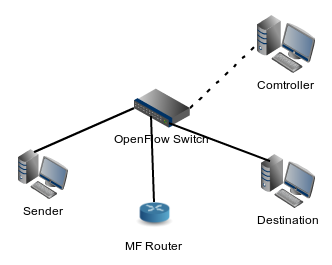
\includegraphics[width=0.3\columnwidth]{images/testcfg2.png}
\end{figure}                                                        

\tableofcontents

\pagebreak

\section{Introduction}

\textbf{HCProbe} is a tool for testing OpenFlow controllers which
includes a library in Haskell providing means to work with OpenFlow
protocol. Also it includes OpenFlow software switch reference
implementation and domain-specific language for constructing new
custom switches.

\subsection{List of terms}

\begin{description}
  \item[OpenFlow] is a communications protocol that gives access to
    the forwarding plane of a network switch or router over the
    network.
  \item[EDSL] embedded domain-specific language
\end{description}

\pagebreak

\section{Subsystems description}

Project HCProbe includes the following subsystems:

\begin{description}
    \item[OpenFlow library] -- OpenFlow protocol implementation
    \item[OpenFlow/Ethernet] -- generation of Ethernet frames
      containing packets from higher level protocols
    \item[HCProbe] -- reference OpenFlow switch implementation
    \item[HCProbe/EDSL] -- domain-specific language for constructing
      OpenFlow software switches
    \item[tests] -- packet generation and parsing tests
    \item[примеры] -- OpenFlow test examples which use switch
      construction EDSL mentioned above
\end{description}


\subsection{OpenFlow library}

OpenFlow library provides OpenFlow protocol implementation in Haskell
based on standard <<OpenFlow Switch Specification, Version 1.0.0>>
\footnote{http://www.openflow.org/documents/openflow-spec-v1.0.0.pdf}.
Main library submodules are:

\begin{description}
    \item[Network.Openflow.Types] -- OpenFlow protocol types and data
      structures
        \begin{itemize}
            \item \textbf{Binary.Read} instances for parsing data
              structures
            \item \textbf{Enum} instances for enumerations
        \end{itemize}
    \item[Network.Openflow.Misc] -- miscellaneous helper functions
        \begin{itemize}
            \item CRC calculation
            \item serialization functions for some types
            \item functions dealing with IP amd MAC addresses
        \end{itemize}
    \item[Network.Openflow.Messages] -- OpenFlow message
      serialization and parsing functions.
\end{description}

\emph{Current implementation is not complete as not 100\% of all
  structures and messages from specification are implented but library
  extension could be done relatively easy by analogy with already
  existing code.}

\subsection{OpenFlow/Ethernet}

This subsystem provides interface for creating packets of different
network protocols (Ethernet, IPv4, ARP, TCP). With its help one could
create custom test packets for incapsulation into PacketIn OpenFlow
messages.

Main modules:

\begin{description}
  \item[Network.Openflow.Ethernet] -- module reexporting all
    submodules (so it suffices to import only this module)
  \item[Network.Openflow.ARP]      -- ARP packets
  \item[Network.Openflow.Frame]    -- network frame (Ethernet)
  \item[Network.Openflow.IPv4]     -- IPv4 packet
  \item[Network.Openflow.TCP]      -- TCP packet
  \item[Network.Openflow.Types]    -- internal data types
\end{description}

hcprobe is an executable implementing a number of software switches
which could be used as a reference implementation of an OpenFlow
switch.

\texttt{hcprobe} program creates some specified number of virtual
switches which connect to a specified controller and after that they
begin to send PacketIn messages to that controller. These messages
contain Ethernet frames with a header including MAC addresses
corresponding to some of virtual switch ports. Also these Ethernet
frames contain IP packet with TCP segment in it.

During program run some statistics is shown on the console. The data
shown include number of sent messages, received messages, mean
roundtrip time for one message and also number of lost messages and
closed connections with controller.

\subsection{EDSL}

Domain-specific language HCProbe was developed for creating OpenFlow
switch programs, for creating different combinations of such switches,
running them and also for registration and collection of statistics on
packet exchange between OpenFlow controller and switches.

\subsubsection{Program structure}

Typical program created using HCProbe domain-specific language
includes at least the following 2 parts:

\begin{itemize}
  \item Switch creation and configuration
  \item Switch run using specified program
\end{itemize}

In most cases 3rd step is required also on which main program thread
waits for switch programs completion (for all or some of them
depending on current task) and calculates summarized statistics.

\subsubsection{Switch creation}

Switch could be created using either \lstinline!switch! or
\lstinline!switchOn! command.  In the first case a switch with default
setting is used as a model. In the second case some previously created
switch could be supplied as a parameter. Thus using command
\lstinline!switchOn! one could create a copy of some already existing
switch.

In order to ensure that MAC address ranges do not overlap between
different switches environment \lstinline!config! should be used in
which switches must be created:

\begin{lstlisting}
    sw <- config $ switch <switchIP> $ do ..
\end{lstlisting}%$

\subsubsection{Configuring switch settings}

Switch configuration is done using environment \lstinline!features! in
which different switch parameters could be specified.

\begin{lstlisting}
    switch <switchIP> $ do
      features $ do
        ..
\end{lstlisting}

These parameters include ports added with \lstinline!addPort! command.

Command \lstinline!addMACs! adds a list of MAC addresses to
switch. And those addresses are equally divided between different
ports of the switch they are assigned to.

\emph{As it was said above to prevent overlapping between MAC
  addresses of different switches environment \lstinline!config! is
  being used. So if during call to \lstinline!addMACs! some
  overlapping with prevously configures switches will be detected then
  instead of these overlapping addresses that switch will be assigned
  other higher an not yet reservec MAC addresses}

\lstinline!clearMACs! clears any MAC addresses assigned to switch.


\subsubsection{Switch run}

Switch could be run in 2 ways:

\begin{itemize}
  \item if standard switch logic is enough for the task it should be
    run using command \lstinline!runSwitch!;
  \item more frequently some custom switch behaviour is needed and it
    could be set up by using command \lstinline!withSwitch!.
\end{itemize}


\subsubsection{Program run}

After switch was started using \lstinline!withSwitch! it begins to
execute some program that was specified. Such program is just an
ordinary block of Haskell code which could work with switch using
special commands for that. These commands include:

\begin{description}
  \item[hangOn] -- wait forever, may be useful in some testing scenarios.

  \item[waitForType] -- waiting for some particular type of message
    from controller: program execution will be suspended till a
    message with specified time arrives, returns message received.

  \item[waitForBID] -- waiting for a message containing specified
    \lstinline!buffer id!.  Returns message received.

\end{description}


For message generation it is desirable that transaction numbers and
buffer ids used in a switch program do not overlap with each
other. To solve this issue commands \lstinline!nextBID! и
\lstinline!nextTID! should be used to get proper ids.

For message sending the following commands could be used:

\begin{description}

  \item[send] -- send arbitrary OpenFlow message to controller

  \item[sendOFPacketIn] -- send OpenFlow message with type
    \lstinline!OFPT_PACKET_IN!

  \item[sendARPGreeting] -- used for sending message
    \lstinline!OFPT_PACKET_IN!  containing ARP reply inside (could be
    used when there is some need to inform controller of all MAC
    addresses available to switch before actuall testings starts)

  \item[statsSend/statsSendOFPacketIn] -- variants of \lstinline!send!
    and \lstinline!sendOFPacketIn! including statistics collection

\end{description}

\subsubsection{Statistics collection}

Current hcprobe implementation supports collection of the following
statistical parameters:

\begin{itemize}
  \item number of sent messages
  \item number of messages for which reply from controller was
    received
  \item number of messages with no reply from controller (messages are
    assumed lost when reply waiting queue gets overflown)
  \item round-trip times from message sending to receiving reply for it
\end{itemize}

Using statistics collection requires the following steps:

\begin{itemize}
  \item \lstinline!initPacketStats! execution to create
    \lstinline!StatsEntity! in which statistics data will be stored
  \item statistics handler regsitration using
    \lstinline!setSilentStatsHandler!  or \lstinline!setStatsHandler stEnt ...!,
    the second call is used e.g. to execute some action where reply
    for a message will be received. Such action could include
    outputting round-trip time to console or file
  \item sending message to controller using commands
    \lstinline!statsSend! or \lstinline!statsSendOFPacketIn!
  \item calculating statistics summary on all controllers using
    command \lstinline!assembleStats!
\end{itemize}

\subsubsection{Setting up custom reaction on controller messages}

In order to switch reaction to controller messages from default one to
some custom reaction (e.g. to check controller reaction on erroneous
switch replies, packet loss etc.) command \lstinline!setUserHandler!
should be used.

\emph{In current implementation statistics collection also uses this
  command so it is not recommended to use both of these mechanisms
  (statistics collection and custom reaction on controller messages)
  at the same time.}

\section{Appendices}

\subsection{Parallel run of software switches}

In order to run one (or more) software switch in parallel with another
and also to control program execution time we use
async\footnote{http://hackage.haskell.org/package/async} library.

The most simple method of using this library is limiting switch
program execution to some specified period of time:

\begin{lstlisting}
import Control.Concurrent (threadDelay)
import Control.Concurrent.Async (race_)

...
race_ action1 (threadDelay 1000000)
\end{lstlisting}

Here we assume that action1 contains start of some switch so the
execution of this line will finish either on switch program
termination (if it does not use default implementation and is finite
in time) or after one second of time.

If more than one switch should be run simultaneously then typical
solution in this case will be to run each of the switches in separate
thread (using \lstinline!async!) and to wait their termination (or
till some period of time expires).

Schematically it will look like:

\begin{lstlisting}
  a1 <- async $ withSwitch sw1 ...
  ...
  aN <- async $ withSwitch swN ...
  mapM_ waitCatch [a1,....,aN]
\end{lstlisting}

If program should be terminated if some error occurs in any of
switches then \lstinline!waitCatch! should be replaced with
\lstinline!wait!.

Instead of \lstinline!withSwitch! command \lstinline!runSwitch! could
be used depending on task required.

\subsection{Program examples}

\subsubsection{Simple switch}

It is one of quite simple examples in which we create 2
switches. Configuration of the second is displayed on the console and
the first is run with default program with time limitation of 3 seconds.

\begin{lstlisting}
{-# LANGUAGE OverloadedStrings #-}
module Main
  where

import Control.Concurrent (threadDelay)
import Control.Concurrent.Async (race_) -- EDSL for asynchronous actions
import Data.Bits                        -- for IP creation
import HCProbe.EDSL

main = do 
    let ip = 15 .|. (0x10 `shiftL` 24)
    (sw1,sw2) <- config $ do
      sw1 <- switch ip $ do
            features $ do
                {- replicateM 48 $ --uncomment to create 48 ports -}
                addPort [] [] [OFPPF_1GB_FD, OFPPF_COPPER] def
                addPort [] [] [OFPPF_1GB_FD, OFPPF_COPPER] def
            addMACs [1..450]
      sw2 <- switchOn sw1 $ do
                clearMACs 
                addMACs [400..500]
      return (sw1,sw2)
    print sw2
    race_ (runSwitch sw1 "localhost" 6633) (threadDelay 3000000)
\end{lstlisting}

\end{document}
